% \documentclass{beamer}
\documentclass{ctexbeamer} % uncomment this if u want the chinese version

\usepackage{lzaBeamerTheme}

\author[lza]{李子奥}
\title{科研向经验分享}
\subtitle{--- 我只是个讲故事的}
\institute{自动化1903班}
\date{\today}

\begin{document}

\maketitle

\begin{frame}
	\headline{我的大学生活-大一上}
	\begin{itemize}
		\item 对科研感兴趣,参加Dian团队招新,被拒(1/3)
		\item 卷王的诞生
		\begin{itemize}
			\item 百分百延续了高中时的思维,即课内最重要,加权至上。
			\item 科研社团等等,是课内学习的“佐料”,不应当占用大量的时间
			\item 在课内学习以外,没有对课外科研的探索
		\end{itemize}
		\item 自我评价: $100\%$的卷王
	\end{itemize}
\end{frame}

\begin{frame}
	\headline{我的大学生活-大一下}
	\begin{itemize}
		\item 背景:疫情元年(2020),呆在家里上网课
		\item 卷王的反思:把《培养计划》视为大学期间奋斗的方向是否合理?
		\item 卷王的尝试
		\begin{itemize}
			\item 参加联创团队招新,被拒(1/1)
			\item 参加Dian团队招新,被拒(2/3)
			\item 参加魏巍老师的《信息检索》公选课(自然语言处理),顺势加入魏巍老师的实验室
		\end{itemize}
		\item 自我评价:$50\%$的卷王
	\end{itemize}
\end{frame}

\begin{frame}
	\headline{我的大学生活-大二上}
	\begin{itemize}
		\item 矛盾:科研$\uparrow$,加权$\downarrow$;加权$\uparrow$,科研$\downarrow$
		\begin{itemize}
			\item 问题:回望大学4年时,除了加权,还剩下什么?
			\item 结论:不能让加权 - 一个冰冰凉凉的数字成为 4 年的主基调
		\end{itemize}
		\item 频繁逃课去实验室学习,阅读(大量?\hspace{0.1em})论文
		\item 产出不多(研究方向毫无进展),收获颇丰(科研的方法论)
		\item 自我评价:$0\%$的卷王
	\end{itemize}
\end{frame}

\begin{frame}
	\headline{我的大学生活-大二上后的寒假}
	\begin{itemize}
		\item 去书城看书,巧遇《CTF 竞赛权威指南-PWN篇》
		\item 感觉很有趣啊!萌生转行做安全的念头
		\item 这时又有了矛盾 $\cdots$
		\begin{itemize}
			\item NLP: 刚刚踏上正道,非常有望产出论文
			\item Security: 陌生而壁垒高,不可能有所产出,对保研(保外)不利
		\end{itemize}
		\item 做自己感兴趣的事情 -- 转行安全\footnote{做完手里的NLP的事情之后}
	\end{itemize}
	\begin{center}
		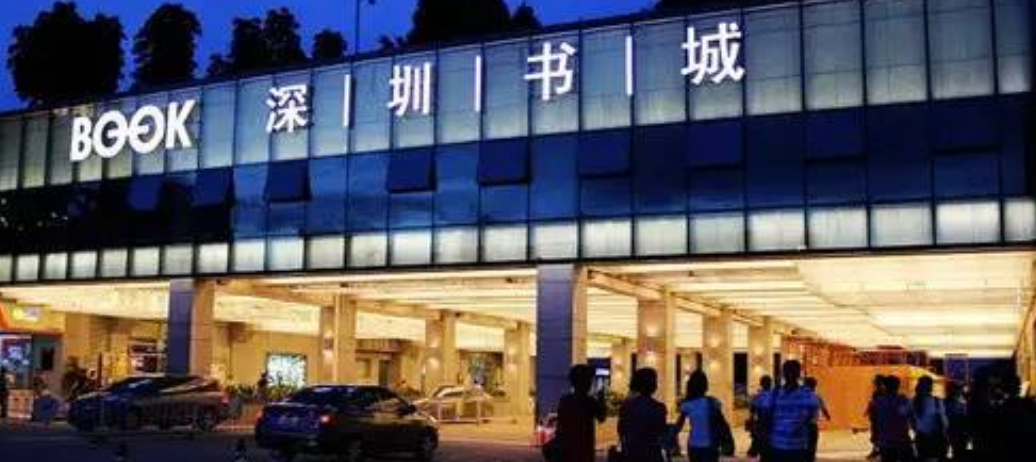
\includegraphics[width=0.6\textwidth]{book}
	\end{center}
\end{frame}

\begin{frame}
	\headline{我的大学生活-大二下}
	\begin{itemize}
		\item 依旧是一个频繁逃课的“坏”学生
		\item 尝试从AI向安全过渡
		\begin{itemize}
			\item 联系网安学院的文明老师
			\item 联系网安学院的付才老师
			\item 参加Dian团队招新,加入网安组(3/3)
		\end{itemize}
		\item 暑假时完成了NLP的工作,产出了一片科(学)研(术)论(垃)文(圾),投稿AAAI,为AI方向画上句话
		\item 自我评价:$0\%$的卷王
	\end{itemize}
\end{frame}

\begin{frame}
	\headline{我的大学生活-大三}
	\begin{itemize}
		\item 联系复旦大学系统安全实验室,远程实习
		\item 不能再当 $0\%$ 的卷王了,不然保研资格无了
		\item 自我评价:$40\%$的卷王
	\end{itemize}
\end{frame}

\begin{frame}
	\begin{center}\Large
	千辛万苦,终于找到并留在自己感兴趣的方向了
	\end{center}
\end{frame}

\begin{frame}
	\headline{追寻内心之光}
	\begin{itemize}
		\item 是否需要找一个自己感兴趣的方向呢??
		\item 我的心路历程 —— \small{发现感兴趣方向的过程}
		\begin{enumerate}
			\item 课内学习是最重要的,科研什么靠边站
			\item 带着功利心地加入实验室,想赶紧弄出篇paper
			\item 发现自己感兴趣的方向了,切换赛道,来到安全
		\end{enumerate}
		\item 如何找到一个感兴趣的方向呢?
		\begin{itemize}
			\item 多尝试些不同的东西(发现自己感兴趣的方向是一个困难的过程
			\item 激发自己的好奇心
		\end{itemize}
	\end{itemize}
\end{frame}

\begin{frame}[fragile]
	\headline{激发自己的好奇心}
	\lstinputlisting[language=c, title=你的第一个C程序,但你真的懂它吗?]{src/main1.c}
	\pause
	\begin{enumerate}
		\item \texttt{\#include}到底有什么用呢?
		\item 我们调用了\texttt{printf}函数,但它的源代码在哪里呢?
		\item $\cdots$
	\end{enumerate}
\end{frame}

\begin{frame}[fragile]
	\headline{激发自己的好奇心 - 神奇的\texttt{printf}}
	\lstinputlisting[language=c, title=将\texttt{\#include<stdio.h>}去掉,它还能运行吗?]{src/main2.c}

	\lstinputlisting[language=c, title=居然能成功运行!但是...有warning]{src/result_main2.txt}
	
	\begin{itemize}
		\item \texttt{warning}说 \texttt{<stdio.h>}提供了对\texttt{printf}函数的声明
		\item 那我们能不能自己加上对 \texttt{printf} 声明呢?
	\end{itemize}
\end{frame}

\begin{frame}[fragile]
	\headline{激发自己的好奇心 - 神奇的\texttt{printf}}
	\lstinputlisting[language=c, title=加上从\texttt{stdio.h}里面找到\texttt{printf}函数的声明\footnote{Borland C选手可以在\texttt{/BC31/DISK\_C/BORLANDC/INCLUDE/STDIO.H}中找到}]{src/main3.c}

	\begin{itemize}
		\item 成功运行!并且\texttt{0 error 0 warning}
		\item 那么,\texttt{printf}的定义(源代码)又在那里呢?
		\item 我们能不能自己加上对\texttt{printf}的定义呢?
	\end{itemize}
\end{frame}

\begin{frame}[fragile]
	\headline{激发自己的好奇心 - 神奇的\texttt{printf}}
	\lstinputlisting[language=c, title=加上对\texttt{printf}函数的定义(源代码)]{src/main4.c}

	\begin{itemize}
		\item 猜猜看会输出什么呢?\pause
		\item 为什么只输出了第一个\texttt{printf}???
		\item 我迫切地想知道原因,我应该如何下手?
	\end{itemize}
\end{frame}

\begin{frame}
	\headline{如果要有建议的话(科研向)- 信息检索篇}
	\begin{itemize}
		\item 人人都要会魔法:魔法能让你检索到你需要的知识(Google/Github/StackOverflow/ChatGPT)
	\end{itemize}
	\begin{center}
		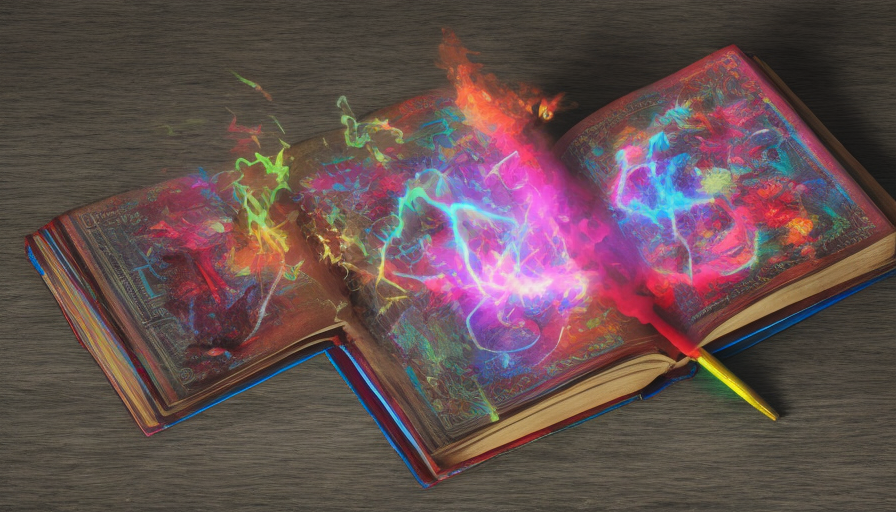
\includegraphics[width=0.7\textwidth]{magic}\\
		\small{Generated By Stable Difussion}
	\end{center}
\end{frame}

\begin{frame}
	\headline{如果要有建议的话(科研向)- 信息检索篇}
	\begin{center}
		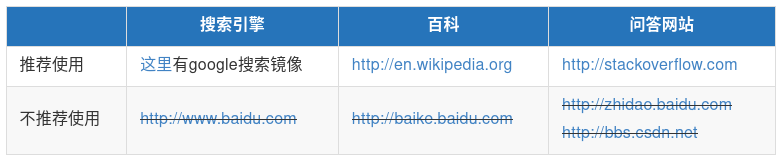
\includegraphics[width=\textwidth]{information}\\
		\small{\href{https://nju-projectn.github.io/ics-pa-gitbook/ics2020/\#\%E6\%90\%9C\%E7\%B4\%A2\%E5\%BC\%95\%E6\%93\%8E-\%E7\%99\%BE\%E7\%A7\%91\%E5\%92\%8C\%E9\%97\%AE\%E7\%AD\%94\%E7\%BD\%91\%E7\%AB\%99}{搜索引擎, 百科和问答网站}}
	\end{center}
	\begin{itemize}
		\item 在提问之前,先RTFM和STFW(\href{https://github.com/ryanhanwu/How-To-Ask-Questions-The-Smart-Way/blob/main/README-zh_CN.md\#rtfm-\%E5\%92\%8C-stfw\%E5\%A6\%82\%E4\%BD\%95\%E7\%9F\%A5\%E9\%81\%93\%E4\%BD\%A0\%E5\%B7\%B2\%E5\%AE\%8C\%E5\%85\%A8\%E6\%90\%9E\%E7\%A0\%B8\%E4\%BA\%86}{提问的智慧的一部分})
		\item 关于如何提问,强烈推荐阅读\href{https://github.com/ryanhanwu/How-To-Ask-Questions-The-Smart-Way/blob/main/README-zh_CN.md}{提问的智慧}和\href{https://github.com/tangx/Stop-Ask-Questions-The-Stupid-Ways/blob/master/README.md}{别像弱智一样提问}
	\end{itemize}
\end{frame}

\begin{frame}
	\headline{如果要有建议的话(科研向)- 信息检索篇}
	\begin{columns}[T,onlytextwidth]
	\column{0.4\textwidth}
		\begin{center}
			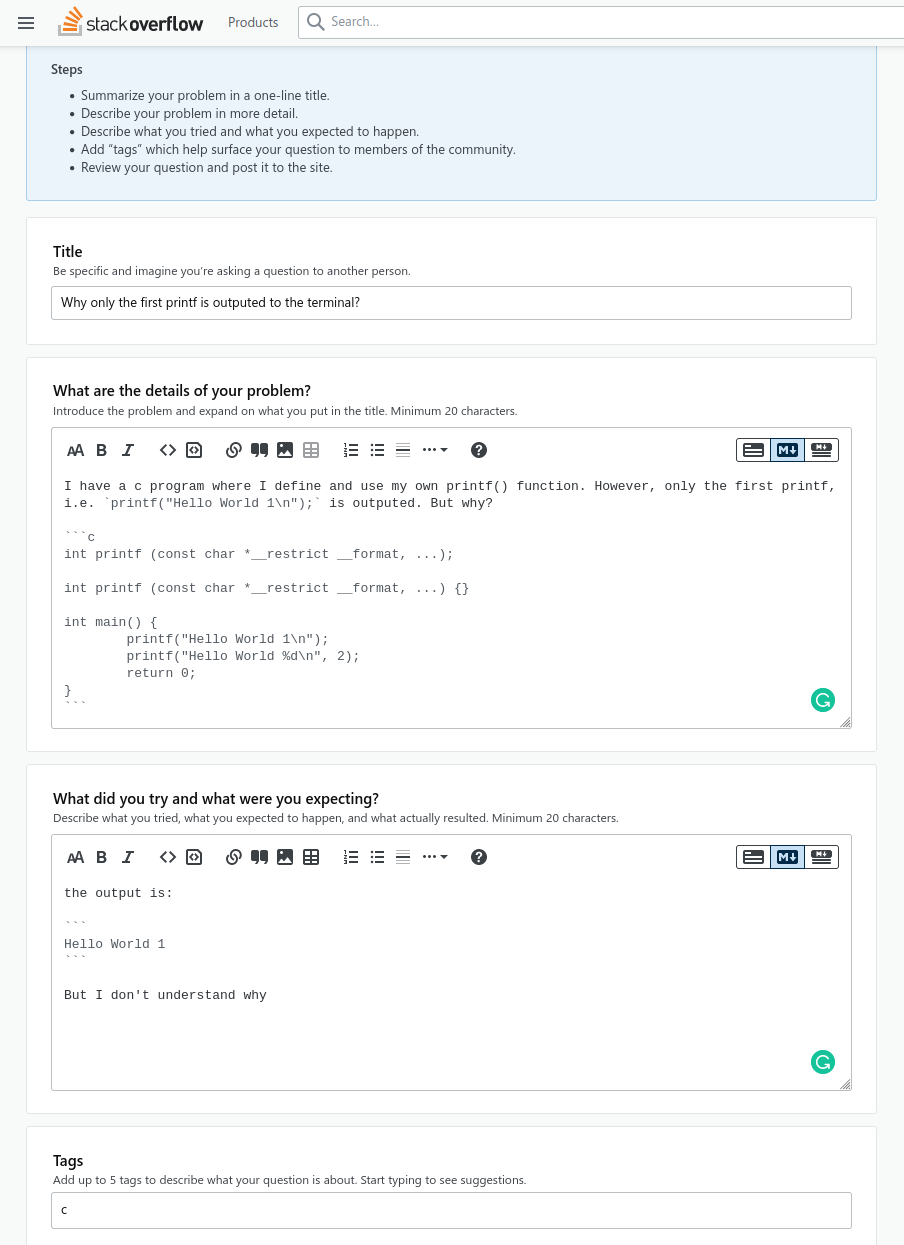
\includegraphics[width=\textwidth]{question}\\
			\small{我在StackOverflow上面提出了这个问题}
		\end{center}
	\column{0.5\textwidth}
		\begin{center}
			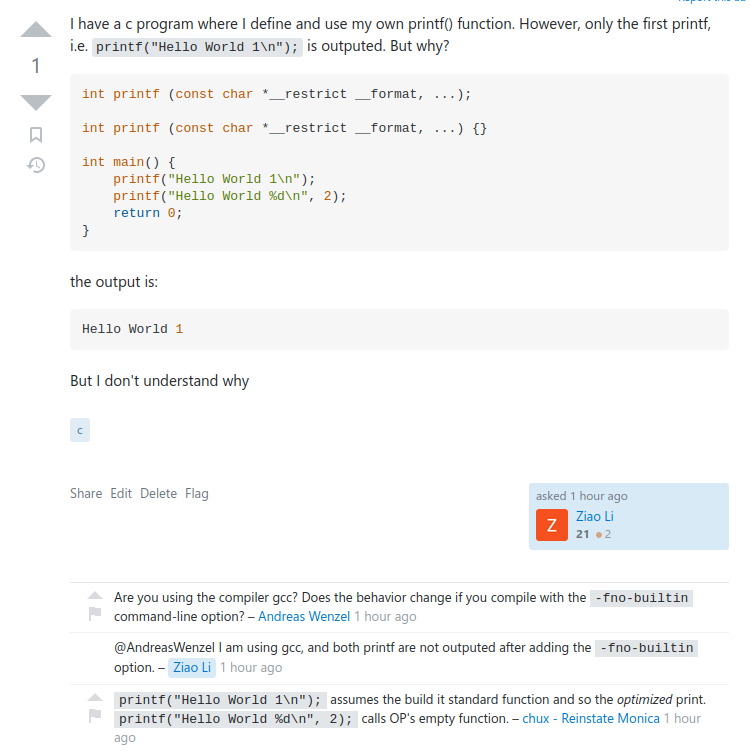
\includegraphics[width=\textwidth]{answer}\\
			\small{很快就收到了\href{https://stackoverflow.com/questions/75851718/why-only-the-first-printf-is-outputed-to-the-terminal}{回复}}
		\end{center}
	\end{columns}
\end{frame}

\begin{frame}
	\headline{如果要有建议的话(科研向)- 实用工具}
	\begin{itemize}
		\item Linux:每个CSer(AIAer)都应该会点Linux,推荐从wsl开始
		\item 笔记软件:推荐obsidian
		\item 论文管理及阅读软件:推荐zotero
		\item 画图软件:PPT/visio/draw.io
	\end{itemize}
\end{frame}

\begin{frame}
	\headline{兴趣是需要被不断激发的}
	\begin{flushright}
		——需要一个好老师的引导
	\end{flushright}
	\begin{itemize}
		\item \href{https://www.bilibili.com/video/BV1iW411d7hd/}{CSAPP}:一个C程序是怎么变成可执行文件的/如何当一个黑客(攻破软件)/网络通信的原理及实现(每个CSer都应该看)
		\item \href{https://www.bilibili.com/video/BV1x7411H7wa/}{The Missing Semester of Your CS Education}:一些cs的基础。我没看过但大伙一致推荐
		\item \href{https://space.bilibili.com/202224425/channel/collectiondetail?sid=192498}{操作系统:设计与实现}:(虽然)讲的是操作系统但是讲的特别有意思
		\item \href{https://www.acwing.com/}{AcWing}:如果你要学算法(Leetcode)不妨从这里开始(收费)
	\end{itemize}
\end{frame}

{
\setbeamercolor{background canvas}{bg=yellow!10}
\begin{frame}
	\headline{联系方式}
	\begin{center}
		
\includegraphics[width=0.3\textwidth]{qq}\\
		\vskip 2ex
		\begin{tabular}{lll}
			姓名 & : & 李子奥 \\
			QQ & : & 2293485914 \\
			Email & : & leeziao0331@gmail.com \\
		\end{tabular}
	\end{center}
\end{frame}
}

% \begin{frame}
% 	\headline{This is another Frame Title}
% 	\begin{columns}
% 	\column{0.5\textwidth}
% 	\begin{block}{Block}
% 		Content of Block
% 	\end{block}
% 	\begin{exampleblock}{Example Block}
% 		Content of Example Block
% 	\end{exampleblock}
% 	\begin{alertblock}{Alert Block}
% 		Content of Alert Block
% 	\end{alertblock}
% 	\column{0.5\textwidth}
% 	\begin{block}{Block}
% 		Content of Block
% 	\end{block}
% 	\begin{exampleblock}{Example Block}
% 		Content of Example Block
% 	\end{exampleblock}
% 	\begin{alertblock}{Alert Block}
% 		Content of Alert Block
% 	\end{alertblock}
% 	\end{columns}
% \end{frame}

\end{document}
